\section{Neural Networks: Regression \& Multinomial Classification}
supervised learning. 
\subsection{Terminology}
\paragraph{Training Example} has form ($x_n, y_n$), with $x_n$ as input vector, $y_n$ expected/true output vector.

\paragraph{Loss/Cost Function} maps values of one or more variables onto a number representing \textbf{loss/cost}.

Learning $\rightarrow$ minimizing a loss function.

\paragraph{Risk Function} \textbf{expectation} of the \textbf{loss function}. In neural network, we minimizes our risk by  \textbf{minimizing the empirical risk function -- average loss of all training examples}.

\paragraph{Activation Function} 
\begin{itemize}
	\item linear activation  
	\item sigmoid activation: \textbf{focus of this lecture},  $\sigma(x) = \frac{e^x}{1 + e^x}$
	\item Perceptron activation
	\item ReLU activation
\end{itemize}
\paragraph{Epoch} one \textbf{forward pass} and one \textbf{backward pass} of \textbf{all} training examples. One pass = forward + backward pass.
\begin{itemize}
	\item Forward Pass: calculate the output of \textbf{all training } through the neural network.
	\item Backward Pass: Backpropagation 
\end{itemize}

\paragraph{Backpropagation} calculate a \textbf{gradient} that is needed in \textbf{calculation of weights} to be used in network. It describes how a \textbf{single training example} starting from \textbf{output neurons} determines the goal for the neurons on the next layer and \textbf{steps backwards recursively}.

\paragraph{Multi-Layer Feed-Forward Networks} represent arbitrary \textbf{non-linear} functions. It consists of
\begin{itemize}
	\item input layer
	\item hidden layer with \textbf{activation}
	\item output layer with \textbf{activation}
\end{itemize}
\textbf{Weights and biases} need to be adapted in the neural network. 

$\rightarrow$ updated by \textbf{backpropagation (gradient descent)}.

\subsection{Multi-Layer Feed-Forward Network}
\subsubsection{Setup of a Neural Network}
\begin{figure}[H]
	\centering
	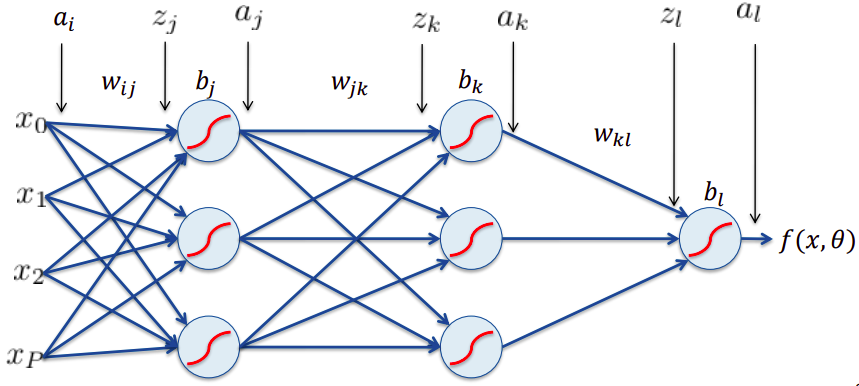
\includegraphics[width=0.7\textwidth]{nn.png}
\end{figure}

\subsubsection{Process}
Goal of training: \textbf{minimizes loss function, minimizes empirical risk}.
\\ \ \\
Assume a network with 1 hidden layer, 1 output layer:

\begin{enumerate}[label= \protect \circled{\arabic*} ]
	\item \textbf{Forward Pass}: from input layer to output layer (with \textbf{sigmoid} activation).
	
	If we are asked to perform, this calculation can done \textbf{matrix-wise}!! No need to separate each observation.
	
	\begin{align*}
		z^{[1]} &= W^{[1]}\cdot a^{[0]} + b^{[1]} =  W^{[1]}\cdot x + b^{[1]}\\
		a^{[1]} &= g^{[1]}(z^{[1]}) = \sigma(z^{[1]}) \\
		z^{[2]} &= W^{[2]}\cdot a^{[1]} + b^{[2]} \\
		a^{[2]} &= g^{[2]}(z^{[2]}) = \sigma(z^{[2]})
	\end{align*}
	
	\item \textbf{Loss Function}: calculate the loss of the network output according to the loss function $l(y, \hat{y})$
	
	If we evaluate the model using \textbf{cross-entropy loss}: the calculation for $y \ln\hat{y}$ is a dot product(element-wise multiplication).
	$$l(y,\hat{y}) = - [y \ln \hat{y} + (1-y)\ln(1 - \hat{y})]$$
	\item \textbf{Empirical Risk}: calculate the empirical risk $\mathcal{L}$ by \textbf{averaging} the loss.
	$$\mathcal{L}(y,\hat{y}) = \frac{1}{n} \cdot \Sigma l(y,\hat{y})$$
	
	\item \textbf{Backpropagation}: readapt the \textbf{weights and biases} using \textbf{gradient descent}. 
	
	example in updating layer 2:
	\begin{align*}
		W^{[2]}_{t+1} &= W^{[2]}_t - \alpha \cdot dW =W^{[2]}_t - \alpha \cdot \frac{\partial L}{\partial W^{[2]}} \\
		b^{[2]}_{t+1} &= b^{[2]}_t - \alpha \cdot db =b^{[2]}_t - \alpha \cdot \frac{\partial L}{\partial b^{[2]}} 
	\end{align*}
	\begin{itemize}
		\item $\frac{\partial L}{\partial W^{[2]}}, \frac{\partial L}{\partial b^{[2]}}$: chain rule
		$$\frac{\partial L_n}{\partial W} = \frac{\partial L_n}{\partial a_{n}} \cdot \frac{\partial a_{n}}{\partial z_{n}} \cdot \frac{\partial z_n}{\partial W}$$
	\end{itemize}
	\begin{align*}
		L_n &= \frac{1}{2} (y_{n} - g(w_{kl}a_{kn} + b_l))^2 = \frac{1}{2} (y_n - a_{ln})^2, \quad &\frac{\partial L_n}{\partial a_{ln}} &= -(y_n - a_{ln})\\
		a_{ln} &= g(z_{ln}) , \quad &\frac{\partial L_n}{\partial z_{ln}} &= g'(z_{ln}) \\
		z_{ln} &= w_{kl}a_{kn} + b_l, \quad &\frac{\partial L_n}{\partial w_{ln}} &= a_{kn} 	
	\end{align*}

	If the activation is a sigmoid activation: $\sigma(x) = \frac{e^x}{1 + e^x}$, $\sigma'(x) = \sigma(x)(1 - \sigma(x))$.
	$$dW^{[2]} = -(y- a^{[2]})\cdot a^{[1]^{T}} = (a^{[2]} - y) \cdot a^{[1]^{T}}$$
\end{enumerate}

\subsubsection{Trainable Parameters}
Number of trainable parameters: the \textbf{free parameters} of the neural network are \textbf{weights and biases}-- $W^{[1]}, b^{[1]}, W^{[2]}, b^{[2]}, \dots$. 

$\rightarrow$ define the \textbf{dimension} of these parameters, add up all possible trainable elements. 

(eg: $W^{[1]}$ is 2x2-matrix, therefore 4 trainable parameters)
\subsection{Gradient Descent for Backpropagation}
\begin{itemize}
	\item Goal: given any function f, find $x^* = \arg\min_{x} f(x)$
	\item \textbf{Gradient} at position x is defined as the \textbf{partial derivative}: 
	$$\nabla f(x) = \begin{bmatrix}
	\frac{\partial f(x)}{x_1} \\ \vdots \\ \frac{\partial f(x)}{x_d}
	\end{bmatrix}$$ 
	\begin{itemize}
		\item Interpretation: in d-dimensional space, gradient points in \textbf{direction of steepest ascent} of f at point x. 	
	\end{itemize}
	$\rightarrow$ to \textbf{minimize loss function} $\rightarrow$ \textbf{descent}, the opposite direction $\mathbf{- \nabla f(x)}$.
	
\end{itemize}
\subsubsection{General Process}
\begin{enumerate}[label= \protect \circled{\arabic*} ]
	\item choose an \textbf{initial point}
	\item choose a \textbf{step size (either fixed or dynamic)}.
	\item take a step in the \textbf{direction opposite the gradient}.
	\begin{itemize}
		\item fixed step size:
		$$\begin{bmatrix}
		x_n \\y_n
		\end{bmatrix} = \begin{bmatrix}
		x_{n-1} \\ y_{n-1}
		\end{bmatrix} - \alpha \cdot \nabla f(x_{n-1}, y_{n-1})$$
		\item dynamic step size:
		$$\begin{bmatrix}
		x_n \\y_n
		\end{bmatrix} = \begin{bmatrix}
		x_{n-1} \\ y_{n-1}
		\end{bmatrix} - \alpha_{n} \cdot \nabla f(x_{n-1}, y_{n-1})$$
	\end{itemize}
	\item repeat till convergence.
\end{enumerate}

Convergence to optimum: depends on the \textbf{step size}. 
\begin{itemize}
	\item too small: would converge eventually, but takes long time.
	\item too large: value \textbf{oscillates}, doesn't converge.
	\item would stall if $\nabla f(x) = 0$. 
	\item can stuck at saddle point.
\end{itemize}
Criteria: 
\begin{itemize}
	\item function f is \textbf{convex}
	\item step size $\alpha$ is square summable, but not summable.
\end{itemize}
$\rightarrow$ Alternative: introduce \textbf{momentum}.

\subsubsection{Process with Momentum Introduced}
\begin{itemize}
	\item Idea: uses an exponential averaging of gradients to \textbf{make sudden changes in direction less likely}.
\end{itemize}
\begin{align*}
	d_n &= \beta \cdot d_{n-1} + \alpha \cdot\nabla f(x_{n-1})\\
	x_n &= x_{n-1} - d_n
\end{align*}
